\documentclass{article}

\usepackage{graphicx}
\usepackage{tikz}
\usepackage{tikzsymbols}
\usetikzlibrary{calc,patterns,shapes.geometric}
\pagestyle{empty}
\usepackage[margin=0pt]{geometry}
\geometry{papersize={14in,12in}}

\def\centerarc[#1](#2)(#3:#4:#5){\draw[#1] ($(#2)+({#5*cos(#3)},{#5*sin(#3)})$) arc (#3:#4:#5);}

\begin{document}
	\begin{figure}
		\centering
		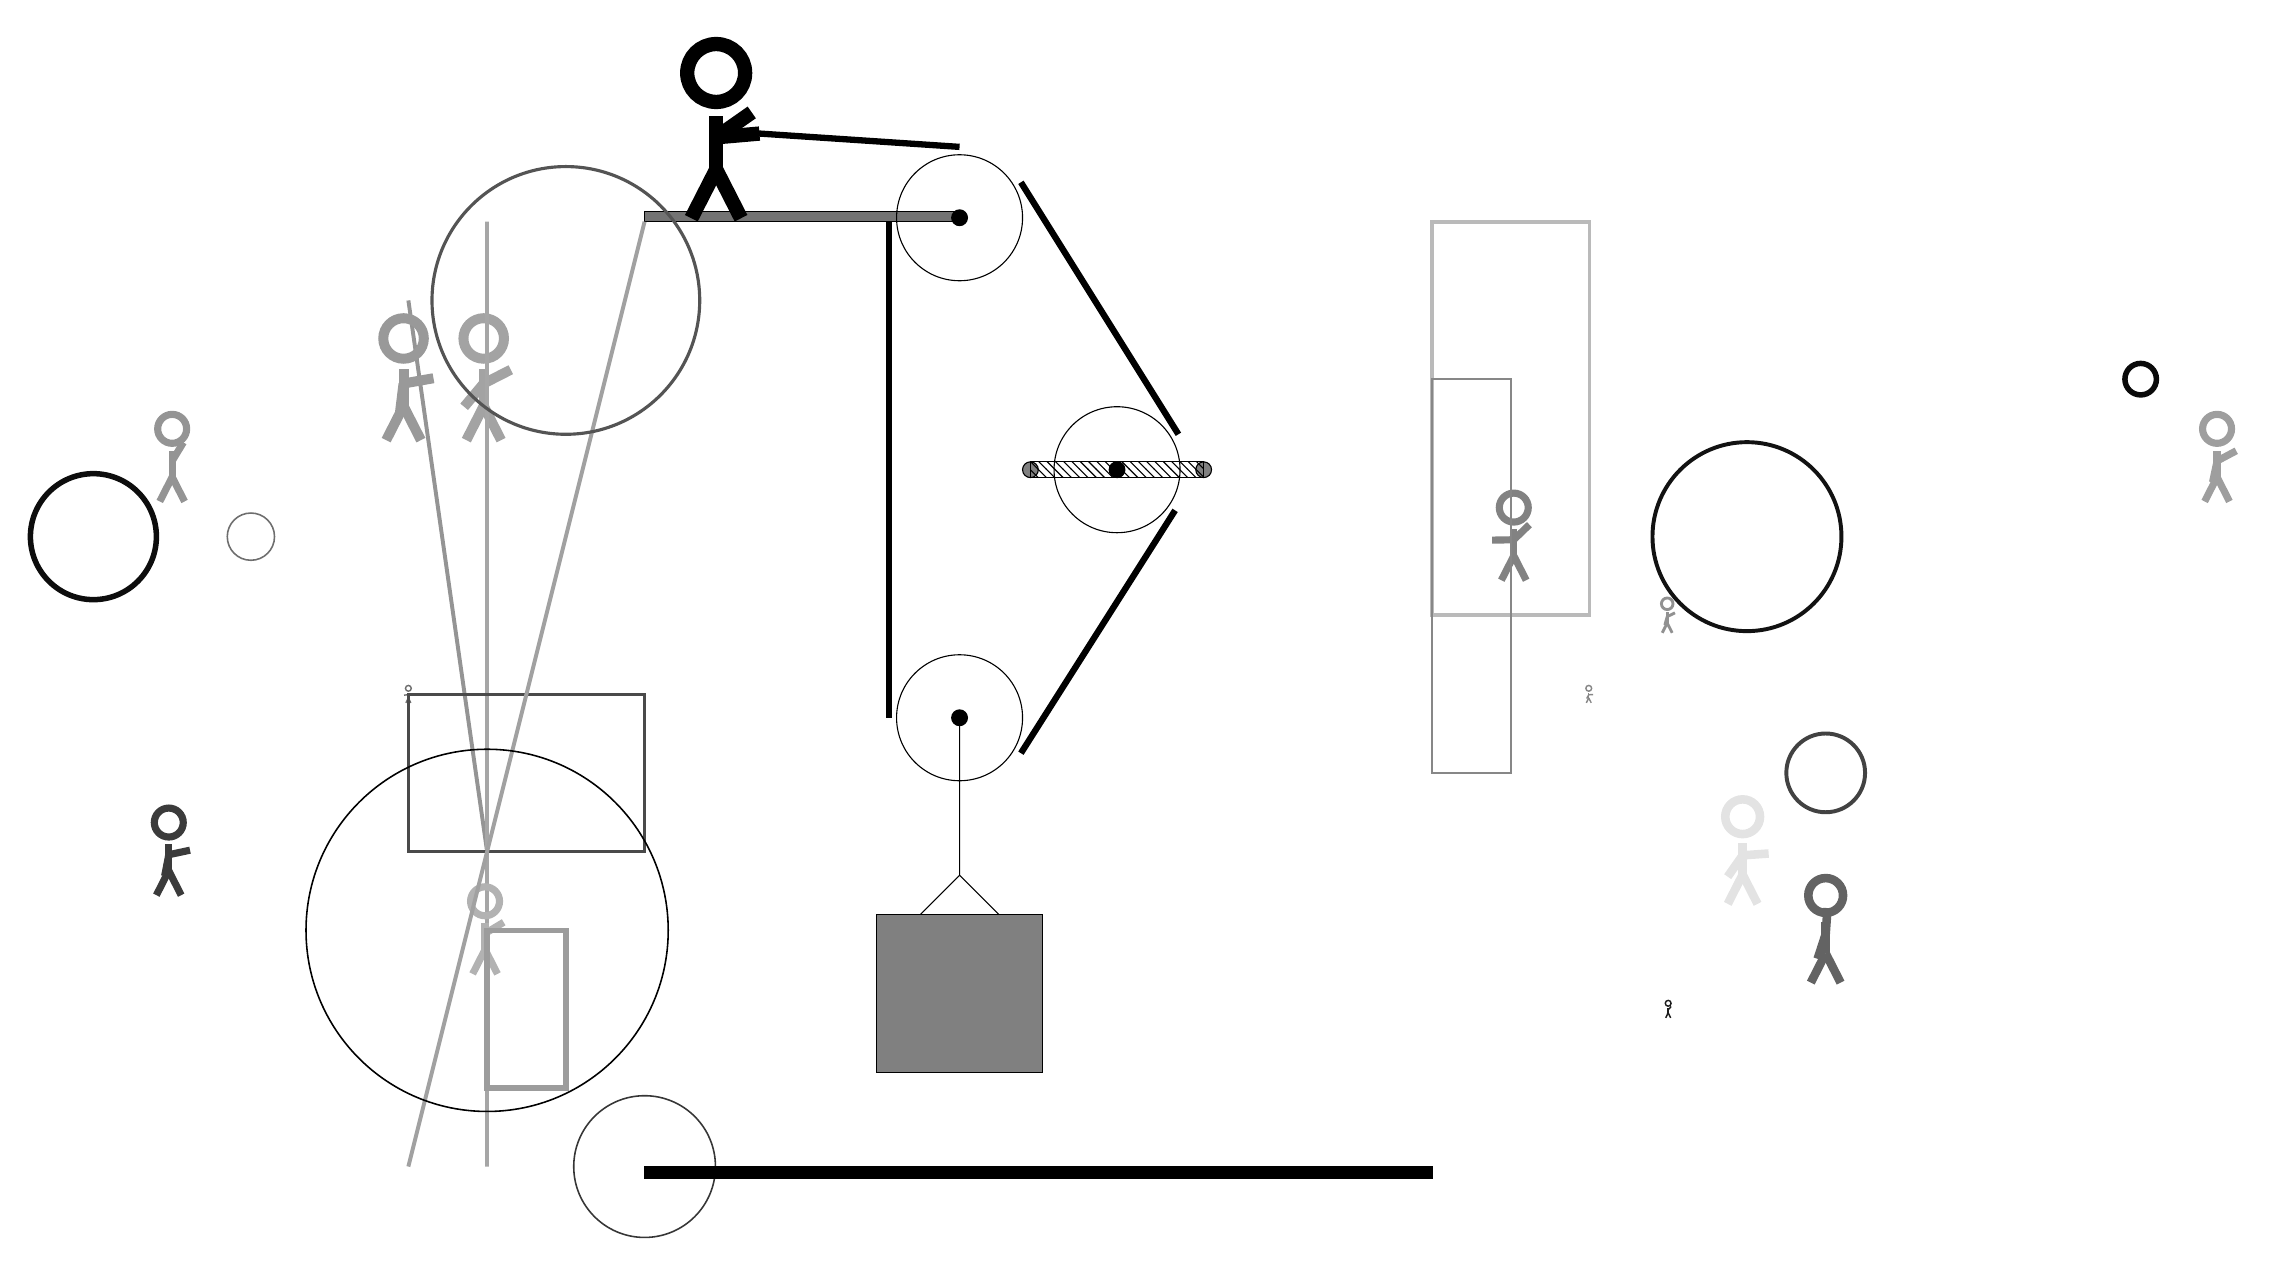
\begin{tikzpicture}
			%%%%% START %%%%%
			
			\draw[fill=black!55] (-2, 9) rectangle (2, 9.125);
			
			\draw[line width=0.5mm, color=black!42](-5, 8) -- (-4, 1);
			
			\node[line width=0.4mm, color=black!36] at (-4, 7) {\Strichmaxerl[7][50][27]};
			\draw[line width=0.5mm, color=black!35] (-4, 9) rectangle (-4, -3);
			\node[line width=0.5mm, color=black!77] at (-8, 1) {\Strichmaxerl[5][79][12]};
			
			\draw [line width=0.2mm, color=black!79](-2, -3) circle (0.9);
			\draw [line width=0.7mm, color=black!96](17, 7) circle (0.2);
			\node[line width=0.6mm, color=black!30] at (-4, 0) {\Strichmaxerl[5][89][31]};
			\draw [line width=0.5mm, color=black!74](13, 2) circle (0.5);
			\node[line width=0.4mm, color=black!57] at (-5, 3) {\Strichmaxerl[1][5][3]};
			
			\node[line width=0.4mm, color=black!49] at (9, 5) {\Strichmaxerl[5][1][44]};
			
			\draw [line width=0.2mm, color=black!57](-7, 5) circle (0.3);
			\draw[line width=0.6mm, color=black!24] (-3, -2) rectangle (-4, 0);
			\node[line width=0.6mm, color=black!89] at (11, -1) {\Strichmaxerl[1][82][47]};
			\node[line width=0.7mm, color=black!40] at (-5, 7) {\Strichmaxerl[7][83][10]};
			\node[line width=0.3mm, color=black!11] at (12, 1) {\Strichmaxerl[6][55][4]};
			\draw [line width=0.7mm, color=black!95](-9, 5) circle (0.8);
			
			\node[line width=0.7mm, color=black!42] at (-8, 6) {\Strichmaxerl[5][90][59]};
			\draw[line width=0.5mm, color=black!27] (8, 4) rectangle (10, 9);
			\node[line width=0.6mm, color=black!38] at (18, 6) {\Strichmaxerl[5][78][28]};
			
			\draw[line width=0.4mm, color=black!71] (-2, 3) rectangle (-5, 1);
			\draw[line width=0.5mm, color=black!37](-2, 9) -- (-5, -3);
			
			\node[line width=0.2mm, color=black!43] at (11, 4) {\Strichmaxerl[2][74][26]};
			
			\draw[line width=0.3mm, color=black!47] (9, 2) rectangle (8, 7);
			\draw[line width=0.7mm, color=black!39] (-3, -2) rectangle (-4, 0);
			\draw [line width=0.5mm, color=black!93](12, 5) circle (1.2);
			\draw [line width=0.2mm, color=black!100](-4, 0) circle (2.3);
			\node[line width=0.4mm, color=black!47] at (10, 3) {\Strichmaxerl[1][61][2]};
			\draw [line width=0.4mm, color=black!67](-3, 8) circle (1.7);
			
			\node[line width=0.7mm, color=black!61] at (13, 0) {\Strichmaxerl[6][72][86]};
			
			
			\draw (2, 2.7) circle (0.8);
			\draw[fill=black] (2, 2.7) circle (0.1);
			
			\draw (2, 9.05) circle (0.8);
			\draw[fill=black] (2, 9.05) circle (0.1);
			
			\draw[fill=white](4, 5.85) circle (0.8);
			\draw[fill=black] (4, 5.85) circle (0.1);
			\draw[fill=black!50] (2.9, 5.85) circle (0.1);
			\draw[fill=black!50] (5.1, 5.85) circle (0.1);
			\draw[pattern=north west lines, pattern color=black] (2.9, 5.95) rectangle (5.1, 5.75);
			
			\draw (2, 2.7) -- (2, 0.7) -- (1.5, 0.2) -- (2.5, 0.2) -- (2, 0.7);
			\draw[fill=black!50] (0.95, 0.2) rectangle (3.05, -1.8);
			
			\draw[line width=0.8mm] (1.1, 9) -- (1.1, 2.7);
			\centerarc[line width=0.8mm](2, 2.7)(180:330:0.9);
			\draw[line width=0.8mm](2.7794, 2.25) -- (4.7373, 5.3338);
			\centerarc[line width=0.8mm](4, 5.85)(390:325:0.9);
			\draw[line width=0.8mm](4.7794, 6.3) -- (2.7794, 9.5);
			\centerarc[line width=0.8mm](2, 9.05)(30:90:0.9);
			\draw[line width=0.8mm](2, 9.95) -- (-1, 10.15);
			
			\node at (-1, 10.15) {\Strichmaxerl[10][-175][35]};
			
			\draw[fill=black] (-2, -3) rectangle (8, -3.15);
			
			%%%%% END %%%%%
		\end{tikzpicture}
	\end{figure}	
\end{document}